% The finish dial. Build: tectonic paper.tex (figures: figs.py; every number: facts.json)
\documentclass[10pt]{article}
\usepackage[letterpaper,margin=1.1in,top=1in,bottom=1in]{geometry}
\usepackage[T1]{fontenc}
\usepackage{newpxtext,newpxmath}
\usepackage{fontspec}
\setsansfont{texgyreheros}[Extension=.otf,UprightFont=*-regular,BoldFont=*-bold,ItalicFont=*-italic,BoldItalicFont=*-bolditalic,Scale=MatchUppercase]
\usepackage{microtype,graphicx,booktabs,xcolor,titlesec,enumitem}
\usepackage[font=small,labelfont=bf,skip=6pt]{caption}
\usepackage[numbers,sort&compress]{natbib}
\setlength{\bibsep}{2pt}
\definecolor{link}{HTML}{1D4ED8}
\usepackage[colorlinks,allcolors=link]{hyperref}
\titleformat{\section}{\sffamily\bfseries\large}{\thesection}{0.6em}{}
\titleformat{\subsection}{\sffamily\bfseries\normalsize}{\thesubsection}{0.6em}{}
\titlespacing*{\section}{0pt}{1.1em}{0.35em}
\titlespacing*{\subsection}{0pt}{0.8em}{0.25em}
\setlength{\parskip}{0.45em}\setlength{\parindent}{0pt}
\setlist{nosep,leftmargin=1.4em}
\newcommand{\ci}[2]{$[#1,\,#2]$}
\newcommand{\x}{$\times$}
\frenchspacing

\begin{document}

\begin{center}
{\sffamily\bfseries\LARGE The Finish Dial\par}
\vspace{0.4em}
{\sffamily\large The top singular directions of an RL weight update\\ set how often a language model finishes its answer\par}
\vspace{1.0em}
{\large The Invariant Swarm}\\[0.25em]
{\small \href{https://monitor.invariant.team}{monitor.invariant.team} \quad$\cdot$\quad November 2026}
\end{center}

\vspace{0.2em}
\begin{center}\begin{minipage}{0.88\textwidth}
\small
{\sffamily\bfseries Abstract.}
Reinforcement learning (RL) with verifiable rewards improves a base model at mathematics, and a few singular
directions of the weight change are known to carry most of that gain. We ask what those directions do to an answer.
In Olmo~3~7B we take the weight change from the base model to the RL model (Olmo~3.1 RL-Zero Math), keep its top 8
singular directions in each weight matrix, and add them to the base at a size we vary from $-1$ to $3$. The base
and every edit of it answer after a prefilled three-token opening (the cue), which by itself recovers much of the RL
gain; every gain we report is on top of the cue. On 328 hard competition problems the size sets how often the model
finishes within its 16{,}384-token limit: 96 answers are cut off at size~$-1$, 77 at size~0 (the base), 46 at
size~1 and 5 at size~2. A random edit with the same singular values stays between 67 and 79 at the four sizes tested,
and removing the directions from the RL model raises its cut-off answers from 25 to 90, near the base's 77. At size
1.5, the best of seven sizes on these problems, the edited base matches the RL model's mean score over four samples
(200.3 against 200.0 right of 328) and trails it under a plurality vote over the four samples (214 against 221).
The edit is computed from the RL model's weights, so it does not replace the RL run; it describes what the top
directions of this run do. They set how often the model finishes an answer, and they also raise correctness, by
less: from the base up to size 1.5 the share of finished answers that are right stays between 60 and 67\,\%
because right answers rise from 161 to 184 on the 251 problems the base already finishes.
\end{minipage}\end{center}
\vspace{0.1em}

\begin{figure}[h]
\centering
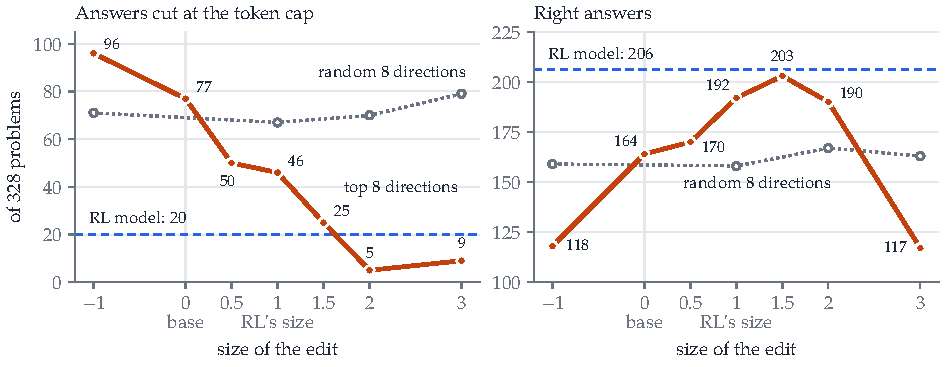
\includegraphics[width=\textwidth]{fig_dial.pdf}
\caption{\textbf{The size of the edit sets how many answers are cut off.} The base model plus \emph{size} \x{}
the top 8 singular directions per matrix of (RL $-$ base), on 328 hard problems, one sample per point.
\textbf{Left:} answers cut off at the 16{,}384-token limit (the cap). \textbf{Right:} right answers. Dotted: the
same edit with random directions. Dashed: the RL model, one sample at the same seed (over five runs it has 190 to
209 right and 20 to 35 cut off). Between repeated runs of one model, right answers vary by 10 to 19 problems.}
\label{fig:dial}
\end{figure}

\section{Introduction}

A model trained with reinforcement learning from verifiable rewards (RLVR) \cite{shao2024deepseekmath,guo2025deepseek}
differs from its base by a small weight change, and that change is close to low rank: one or a few singular
directions per matrix recover most of the accuracy gain \cite{cai2025predictability,wei2026minimal,ye2026implicit}.
We ask what those directions do to an answer.

An answer to a hard problem can fail in two ways: the model writes until the token limit and never commits (the
answer is \emph{cut off}), or it finishes with a wrong answer. So accuracy is, to within a few answers, a product:
$\text{right} = \text{finished} \times \text{right among finished}$,
and an edit can move either factor. We scale the low-rank part of the RL update up and down and read both
(Figure~\ref{fig:dial}). The size of the edit moves the first factor over almost its whole range, in both
directions, and a random edit of the same size moves neither. The second factor, which we call precision, is measured on a different
set of answers at each size, so we also count right answers on the fixed set of problems the base already finishes. We claim
that the top directions control how often the model finishes: cut-off answers fall monotonically up to size 2, and random
directions with the same singular values do not have this effect. We do not claim that they leave correctness untouched; they
also raise it, by less.

\section{Setup}

\textbf{Models.} All models are 7B checkpoints of the Olmo~3 family \cite{ettinger2025olmo} and share one base:
Olmo~3 Base; \emph{RL}, the Olmo~3.1 RL-Zero Math checkpoint, trained from the base with RLVR and no
demonstrations; and \emph{Think-SFT}, the Olmo~3 Think SFT checkpoint, trained from the base by supervised
fine-tuning on reasoning traces, with no reward.

\textbf{Problems.} 328 competition problems (AIME 2022--2025, AMC, HMMT, OlympiadBench): a pool of 400 minus the 72
we found, exactly or nearly, in the RL model's training prompts. We also report MATH-500, the 500-problem subset
\cite{lightman2023lets} of the MATH test set \cite{hendrycks2021measuring}. We sample at temperature 1.0 with at
most 16{,}384 new tokens; an answer that reaches this limit is cut off. An answer is right if its last boxed
expression or \texttt{Answer:} line is equivalent to the reference; a few cut answers are right this way (3 of the
base's 77).

\textbf{Prompt.} Fixing the first tokens of the response recovers much of the RL gain on this base
\cite{wang2026base}. The base, every edit of it and Think-SFT therefore start from a three-token prefilled opening
ending in ``Okay'', which we call the cue (ours is \texttt{`` line!\textbackslash n\textbackslash nOkay''}; that
paper uses a two-token one). Every gain below is on top of the cue. The RL model runs without the cue. With the
cue it scores the same: 205 right and 25 cut off with the cue, against 206 right and 20 cut off without it (one
sample each).

\textbf{The edit.} Let $D = W_{\mathrm{RL}} - W_{\mathrm{base}}$ for each of the 224 attention and MLP projection
matrices (7 per layer, 32 layers), and $D_8 = U_8 \Sigma_8 V_8^{\top}$ its top 8 singular directions, which hold
9.8\,\% of $\|D\|^2$. The edited model is $W_{\mathrm{base}} + s\,D_8$, with size $s$. The control replaces $U_8$
and $V_8$ by random orthonormal matrices and keeps $\Sigma_8$, so it has the same norm in every matrix. Intervals
are 95\,\% paired bootstrap intervals over problems, in percentage points of 328.

\section{Results}

\subsection{The size of the edit sets how often the model finishes}\label{sec:dial}

Cut-off answers fall as the size grows (Figure~\ref{fig:dial}, left): 96 of 328 at size $-1$, 77 at 0, 50 at 0.5,
46 at 1, 25 at 1.5, 5 at 2 and 9 at size~3; the paired interval of every step up to size 2 except 0.5 to 1 excludes zero. Subtracting the directions makes
the base finish less often than it does untouched; twice the RL amount leaves almost no answer cut off. The
random edit stays between 67 and 79 cut-off answers at sizes $-1$, 1, 2 and~3. Mean answer length changes little (9{,}344
tokens for the base, 8{,}916 at size 1.5), so the edit does not shorten all answers; it ends the ones
that would have run to the limit.

Right answers rise and then fall (Figure~\ref{fig:dial}, right): 164 for the base, 192 at size 1, 203 at size 1.5,
190 at size 2, and 117 at size 3, where only 36.4\,\% of finished answers are right. At size 1 the edit is $+10.4$ points \ci{5.8}{14.9} above
the random edit of the same size, and at size 2 it is $+7.0$ \ci{2.7}{11.3} above.

Between sizes 0 and 1.5 the share of finished answers that are right stays between 60 and 67\,\% (64.1\,\% for the
base, 66.3\,\% at 1.5). This is not because the edit leaves correctness alone. At size 1.5, 64 of the base's 77
cut-off answers now finish, and only 19 of them are right. These are the harder problems, so an edit that changed
only when the model stops would lower precision.

Precision stays level because right answers on the 251 problems the base already finishes rise from 161
to 184 (random edit: between 149 and 158 at its four sizes, below the base; RL model: 187). Of the net gain of 39
right answers at size 1.5 (203 against 164), 16 are on the 77 problems the base ran to the limit (19 right, against
the base's 3) and 23 on the 251 it already finished. Outside this range precision falls: to 50.9\,\% at size
$-1$, 58.8\,\% at size 2 and 36.4\,\% at size 3. Figure~\ref{fig:plane} shows the same runs with the two factors as
axes.

\begin{figure}[t]
\centering
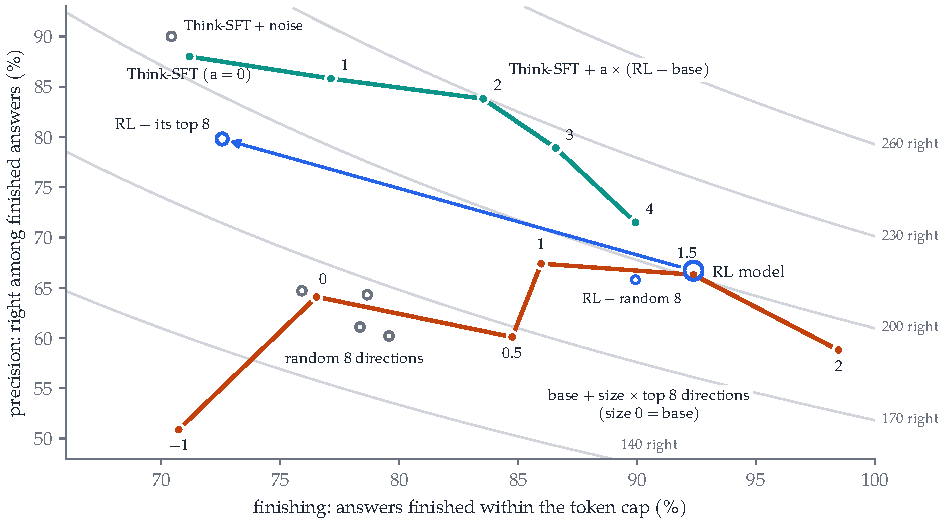
\includegraphics[width=\textwidth]{fig_plane.pdf}
\caption{\textbf{Finishing and precision, one point per model} on the 328 problems. Grey curves join points with
the same number of right answers; up and to the right is better. \textbf{Orange:} the edited base moves mostly to
the right (more answers finished, about the same precision) between sizes 0 and 1.5, where it reaches the RL model,
and loses precision at $-1$ and 2 (size 3, at 97\,\% finished and 36\,\% precision, is off the plot).
\textbf{Blue:} removing the same 8 directions from the RL model moves it left and up: it finishes fewer, easier
problems. Removing 8 random ones (small blue ring) does not. \textbf{Green:} adding $a$ \x{} the whole RL update
to Think-SFT, the model trained by imitation, also raises finishing and lowers precision. Grey rings are the
random-direction and noise controls. The RL model is run with the cue here (205 right, 25 cut off). Orange and
blue points are one sample; green points are means of one to four samples.}
\label{fig:plane}
\end{figure}

\subsection{Without the directions, the RL model finishes no more often than the base}\label{sec:remove}

To test whether the RL model needs the directions, we subtract $D_8$ from the RL model itself and run both with
the cue (one sample each, different seeds). Cut-off answers go from 25 to 90 ($+19.8$ points \ci{15.2}{24.4}),
back to the level of the base (77). Subtracting a random rank-8 matrix with the same singular values leaves 33.
Right answers fall from 205 to 190 ($-4.6$ points \ci{-8.2}{-1.2}), within noise of the random removal (195). The
answers the model still finishes are right 79.8\,\% of the time. They are an easier, self-selected set, because
the long, hard answers are the ones that no longer end.

\subsection{At size 1.5 the edited base matches the RL model's mean score}\label{sec:match}

Size 1.5 was the best of seven sizes on one sample of the 328 problems, so we drew again (Table~\ref{tab:match}). Over four
samples the edited base averages 200.3 right and the RL model 200.0, a difference of $+0.1$ points
\ci{-1.7}{1.8}; the base with the cue averages 158.5. The first of the four samples reuses the seeds of the
original run; the three new draws give 198, 199 and 197. On MATH-500, which played no part in choosing the size,
one sample of the edit scores 456 of 500, equal to the lowest of the RL model's four samples (456 to 464, mean
460.0). Under a plurality vote over the four samples the edit trails the RL model, 214 against 221 ($-2.1$ points
\ci{-5.2}{0.6}).

\begin{table}[h]
\centering\small
\begin{tabular}{@{}lcccc@{}}
\toprule
 & \multicolumn{3}{c}{328 hard problems, four samples} & MATH-500 \\
\cmidrule(lr){2-4}\cmidrule(l){5-5}
Model & right: mean (each sample) & cut off, mean & vote over 4 & right of 500 \\
\midrule
Base + cue & 158.5 \;(161, 161, 152, 160) & 71.5 & 192 & 405--418 \\
Base + cue + 1.5 \x{} $D_8$ & 200.3 \;(207, 198, 199, 197) & 19.0 & 214 & 456 \\
RL model & 200.0 \;(207, 190, 209, 194) & 28.5 & 221 & 456--464 \\
\bottomrule
\end{tabular}
\caption{At size 1.5 the edited base matches the RL model's mean score on the 328 problems and trails it under
a vote over four samples. MATH-500 ranges are over four samples; the edit has one sample.}
\label{tab:match}
\end{table}

\subsection{Directions from five of six RL checkpoints reduce cut-off answers}\label{sec:reward}

The Olmo~3 release has RL-Zero checkpoints trained from the same base on four rewards (math, code, instruction
following and a general mix), in six checkpoints: math and code in versions 3.0 and 3.1, the other two in 3.0. We
built the top-8 edit from each, at size 1 (Table~\ref{tab:reward}). Five of the six reduce cut-off answers, the
instruction-following one included. Only the general one does not, and its edit has half the norm of the math edit,
so this negative result does not compare edits of equal norm. What separates the rewards is the score: Math~3.1
raises it most (192), Math~3.0 and the code checkpoints follow within noise of each other, and instruction following
reduces cut-off answers without raising the score (155, $-2.7$ points \ci{-7.3}{1.5} against the base).

We measure how much two checkpoints share a subspace as $\|V_a^{\top} V_b\|_F^2 / 8$ for their top-8 input
directions, averaged over matrices: 1 for identical subspaces, 0.002 for random ones, and 0.04 between the math
update and the base matrices' own top 8. Two math checkpoints overlap by 0.48, math and code by 0.26, and math with
instruction following by 0.03. The instruction-following edit still reduces cut-off answers, so finishing is not
confined to one subspace.

Rank 1 already gives most of the drop in cut-off answers and about half of the gain in right answers: at size 1,
ranks 1, 8 and 64 give 181, 192 and 200 right (base 164) and 51, 46 and 42 cut off (base 77); rank 64 is above
rank 1 by $+5.8$ points \ci{1.8}{10.1}.

\begin{table}[h]
\centering\small
\begin{tabular}{@{}lcc@{}}
\toprule
Source of the 8 directions & Right of 328 & Cut off \\
\midrule
None (base + cue) & 164 & 77 \\
RL-Zero Math 3.1 (the RL model) & 192 & 46 \\
RL-Zero Math 3.0 & 182 & 43 \\
RL-Zero Code 3.1 & 178 & 41 \\
RL-Zero Code 3.0 & 173 & 23 \\
RL-Zero Instruction following 3.0 & 155 & 41 \\
RL-Zero General 3.0 & 164 & 88 \\
\bottomrule
\end{tabular}
\caption{Directions from five of the six RL checkpoints leave fewer answers cut off than the base; Math~3.1
raises right answers most. The base plus the top 8 directions of each checkpoint, size 1, one sample each.}
\label{tab:reward}
\end{table}

\subsection{The same trade in a model trained by imitation}\label{sec:transplant}

Think-SFT sits at the opposite corner of Figure~\ref{fig:plane}: 88.0\,\% of its finished answers are right, but
it is cut off on a mean of 94.5 of 328 problems over four samples. Its weight change from the base is about 114
times larger in Frobenius norm than the RL update and orthogonal to it (cosine $-0.002$). We add $a$ times the
whole RL update to it. Cut-off answers fall with every step (94.5, 75, 54, 44, 33 for $a = 0$ to 4) and precision falls with them (88.0, 85.8, 83.8, 78.9,
71.5\,\%), so the score peaks in between: 231.5 of 328 at $a = 2$, above Think-SFT (209.0) and the RL model
(200.0). Gaussian noise with the norm of the RL update before rounding to bfloat16 changes nothing (209 right, 97
cut off). That a sum of an imitation model and an RL update can beat both is known \cite{yuan2026decouple}; here
cut-off answers and precision both fall as $a$ grows, which is consistent with the best score lying at an
intermediate $a$. Here the edit is the full update, not its top 8 directions, and
$a = 1$, 3 and 4 are one sample.

\section{Related work}

\textbf{Low-rank RL updates.} The top singular direction of an RLVR update recovers nearly all of its accuracy gain
\cite{cai2025predictability,wei2026minimal,ye2026implicit} and evolves near-linearly over training, so later
checkpoints can be extrapolated from early ones \cite{cai2025predictability,wei2026minimal}; RLVR updates avoid
the principal directions that supervised fine-tuning targets \cite{zhu2025path}. These works report accuracy. We
report what the directions do to an answer, with a random-direction control and a removal test.

\textbf{Scaling weight differences.} Task vectors can be added, negated and scaled \cite{ilharco2022editing};
scaling a fine-tuning update past 1 can improve a model \cite{zheng2024model}; a weight direction between two
code-RL policies controls resource-limit failures \cite{zheng2026correctness}; and an edit of a few attention heads
changes how long a reasoning model thinks \cite{sun2025thinkedit}. Reasoning updates transfer between models
\cite{zbeeb2025reasoning} and combine with imitation updates \cite{yuan2026decouple}.

\textbf{What RL adds.} RLVR
raises accuracy mostly on problems the base can already solve in some samples
\cite{yue2025does,kim2025reinforcement}; part of its reported out-of-domain gain is answer format
\cite{lyu2026same}; and an opening cue recovers much of it \cite{wang2026base}. We add a weight-space account of
one more part: finishing.

\section{Limitations}

\begin{itemize}
\item The edit is computed from the RL model's weights. It explains the RL update; it does not replace the RL~run.
\item We test one model family, at one size (7B), on mathematics only. Each point of Figure~\ref{fig:dial} is one
sample of 328 problems, and right answers vary by 10 to 19 problems between repeated runs of one model, so only the
large contrasts are resolved.
\item Size 1.5 was chosen on the 328 problems. The new samples are on the same problems; MATH-500 is the only other set.
\item The random control was run at sizes $-1$, 1, 2 and 3, not at 0.5 or 1.5.
\item One token limit. At a larger limit fewer answers are cut off, and we have not measured the edit there.
\item The weights are stored in bfloat16, and at these sizes much of the stored edit is rounding noise: at size
1.5 the edit is 0.11\,\% of the weight norm as intended and 0.19\,\% as stored. The random control is rounded the
same way and stays flat, so the effect is not the rounding.
\end{itemize}

\section{Conclusion}

In this model the best-known part of the RL update, its top singular directions, works as a control on committing
to an answer. Scaling them above the RL amount or below zero, or removing them from the RL model, moves the number
of cut-off answers in the matching direction each time. Between sizes 0 and 1.5, cut-off answers fall from 77 to 25
while precision stays between 60 and 67\,\%, which suggests reporting the two separately: a benchmark score at a
fixed token limit mixes how well a model reasons with how readily it~stops.

{\small
\textbf{Reproducibility.} Code, the metrics of every run and the script that draws both figures are in the team's
repository under \texttt{studies/rlneurons/}, which is private and available on request; each number in this paper
is listed with its source in the file \texttt{paper/facts.json} of that folder.
}

{\footnotesize
\bibliographystyle{unsrtnat}
\bibliography{refs}
}
\end{document}
